% -*- coding: utf-8 -*-
% Prezentacja 15 min: predykcja zapchania mlyna weglowego.
% Kompilacja: pdflatex prezentacja.tex (dwa przebiegi). Ryciny w fig/.
\documentclass[aspectratio=169,11pt]{beamer}
\usepackage[utf8]{inputenc}
\usepackage[T1]{fontenc}
\usepackage[polish]{babel}
\usepackage{graphicx}
\usepackage{booktabs}
\usepackage{amsmath,amssymb}
\usepackage{xcolor}
\usepackage{colortbl}

\usetheme{Frankfurt}
\usecolortheme{whale}
\useinnertheme{circles}
\setbeamertemplate{navigation symbols}{}
\setbeamertemplate{footline}[frame number]
\setbeamertemplate{caption}[numbered]
\setbeamercovered{transparent}
\definecolor{akcent}{RGB}{0,90,160}
\setbeamercolor{block title}{bg=akcent!18,fg=black}

% skroty
\newcommand{\sig}[1]{\textcolor{akcent}{\textbf{#1}}}

\title[Predykcja zapchania młyna]{Wczesne ostrzeganie przed zapchaniem młyna węglowego}
\subtitle{Identyfikacja obiektu i model predykcyjny na danych DCS}
\author[Wróblewski, Smardzewski]{Jakub Wróblewski \and Mateusz Smardzewski}
\institute[PW EiTI]{Politechnika Warszawska, Wydz. Elektroniki i Technik Informacyjnych\\Automatyka i Robotyka --- Metody Identyfikacji}
\date{czerwiec 2026}

\begin{document}

\begin{frame}[plain]
  \titlepage
\end{frame}

\begin{frame}{Plan}
  \footnotesize
  \tableofcontents
\end{frame}

% =====================================================================
\section{Problem}

\begin{frame}{Problem --- w jednym zdaniu}
  \begin{block}{Cel}
    Przewidzieć \sig{zapchanie (dławienie) młyna węglowego} z~minutowych danych
    DCS na tyle wcześnie, by zdążyć zareagować przed awaryjnym odcięciem podajnika.
  \end{block}
  \vspace{0.4em}
  \begin{columns}[T]
    \begin{column}{0.54\textwidth}
      \textbf{Dlaczego to ważne} \scriptsize (widownia zna temat)
      \begin{itemize}\footnotesize
        \item zapchanie $\Rightarrow$ spadek wydajności mielenia, wahania mocy bloku,
        \item kończy się \sig{awaryjnym cięciem podajnika} i~odstawieniem młyna,
        \item dziś wykrywane \emph{po fakcie} --- operator reaguje, gdy już dławi.
      \end{itemize}
    \end{column}
    \begin{column}{0.46\textwidth}
      \textbf{Teza projektu}
      \begin{itemize}\footnotesize
        \item prekursory są widoczne \sig{60--120 min} przed kulminacją,
        \item więc jest fizyczna podstawa do \sig{wczesnego ostrzegania},
        \item zadanie: zamienić tę fizykę w~działający alarm.
      \end{itemize}
    \end{column}
  \end{columns}
  \vfill
  {\scriptsize Dane: blok 1, młyny wentylatorowe MW1--MW4, luty 2026, rozdzielczość 1~min.}
\end{frame}

\begin{frame}{Anatomia epizodu --- fizyka, na której stoi rozwiązanie}
  \begin{columns}[T]
    \begin{column}{0.62\textwidth}
      \centering
      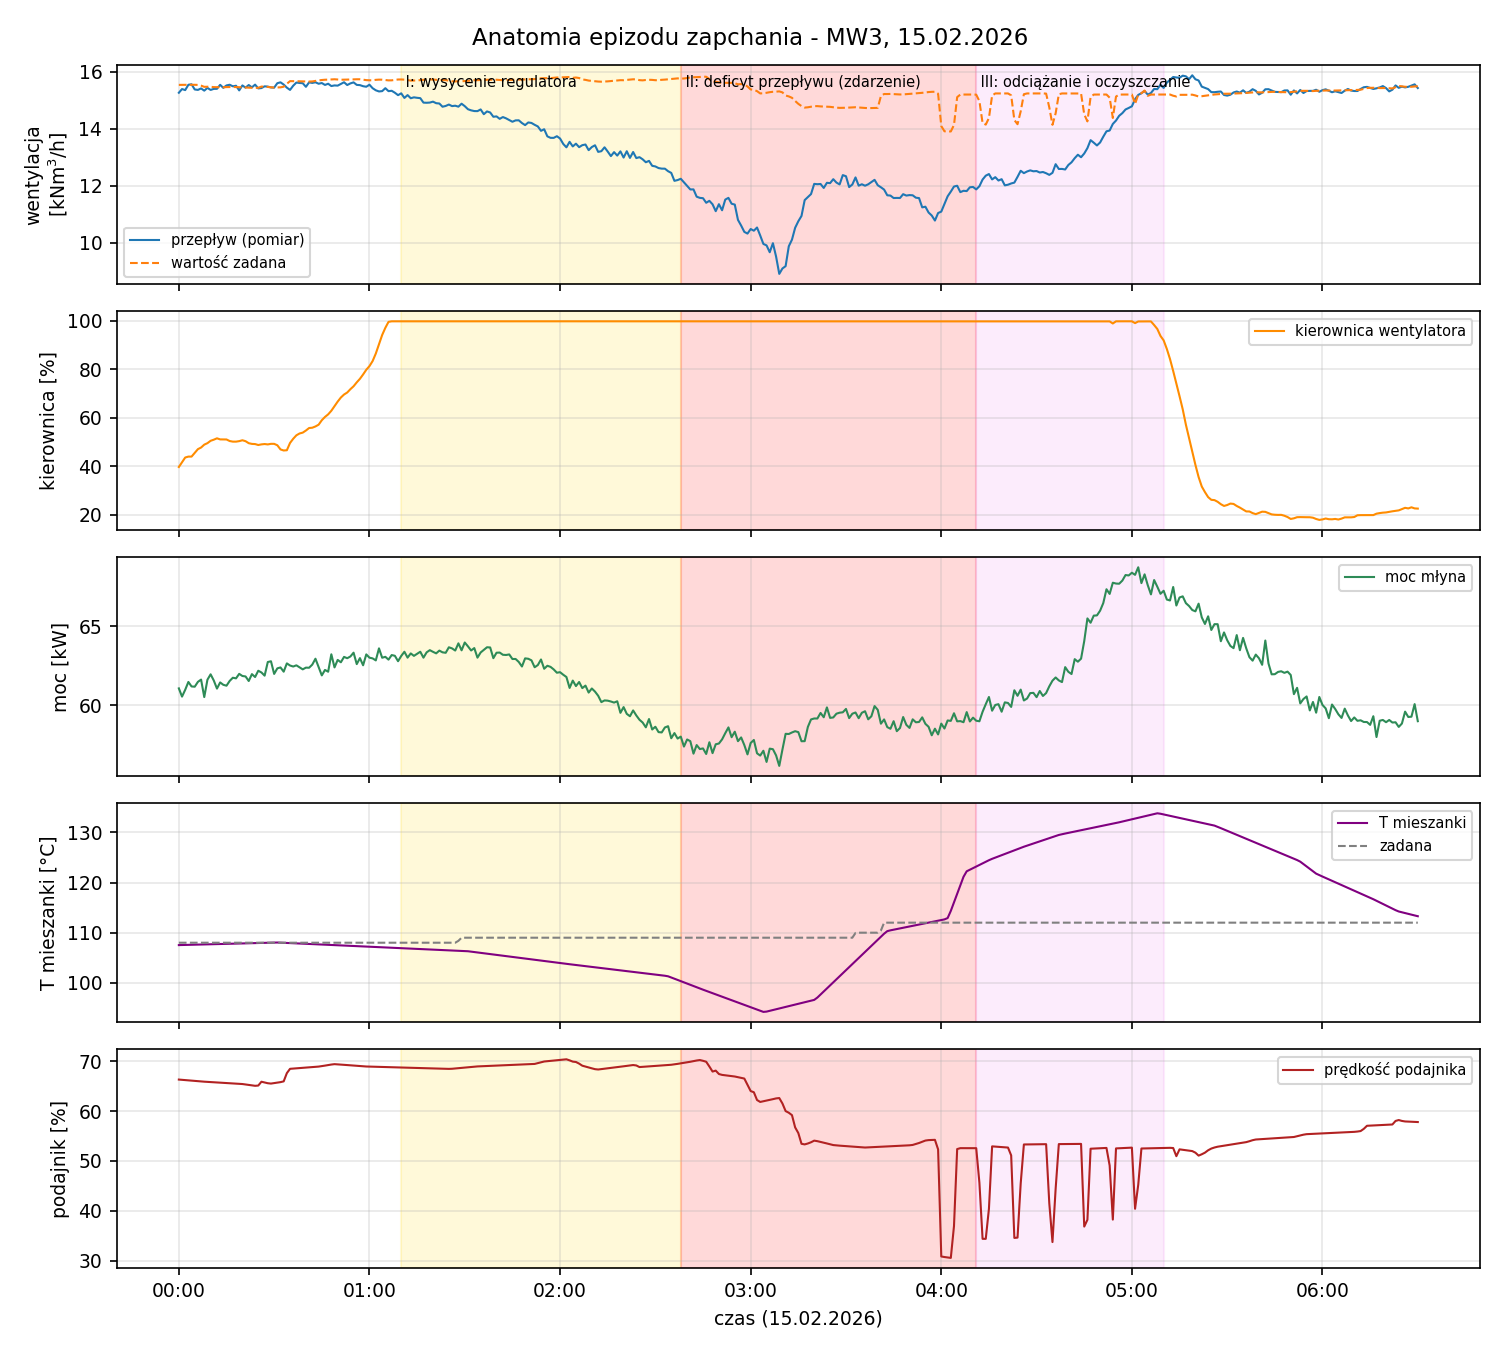
\includegraphics[width=\textwidth,height=0.74\textheight,keepaspectratio]{fig/anatomia_zdarzenia.png}
    \end{column}
    \begin{column}{0.38\textwidth}
      \footnotesize Powtarzalna sekwencja (MW3, 15.02):
      \begin{enumerate}\footnotesize
        \item regulator wentylacji otwiera kierownicę aż do \sig{wysycenia 100\%},
        \item mimo to \sig{przepływ spada} poniżej zadanego (rośnie opór),
        \item \sig{moc młyna rośnie}, temperatura mieszanki spada,
        \item automatyka \sig{awaryjnie tnie podajnik} --- młyn się oczyszcza.
      \end{enumerate}
      \vspace{0.3em}
      To \emph{kierowany} proces fizyczny, a nie szum --- dlatego daje się go modelować.
    \end{column}
  \end{columns}
\end{frame}

% =====================================================================
\section{Dane i~definicja zdarzenia}

\begin{frame}{Dane --- krótko}
  \begin{columns}[T]
    \begin{column}{0.5\textwidth}
      \textbf{Co mamy}
      \begin{itemize}\footnotesize
        \item 4 młyny $\times \sim$38 sygnałów, 1 min, 01--27.02,
        \item $\sim$37\,440 minut/młyn ($\sim$40 MB),
        \item sygnały kluczowe: regulacja wentylacji (pomiar/zadana/sterowanie), moc młyna, podajnik, temperatura mieszanki.
      \end{itemize}
    \end{column}
    \begin{column}{0.5\textwidth}
      \textbf{Pułapki (obsłużone w \texttt{loader.py})}
      \begin{itemize}\footnotesize
        \item kodowanie cp1250,
        \item \sig{mieszane formaty czasu} w jednym pliku,
        \item braki \texttt{N\_A}/\texttt{NaN} ($\sim$3\%).
      \end{itemize}
    \end{column}
  \end{columns}
  \vspace{0.6em}
  \begin{block}{Kluczowy fakt}
    \footnotesize Brak dziennika zdarzeń DCS $\Rightarrow$ \sig{zdarzenia trzeba zdefiniować sygnałowo}.
    W~lutym wszystkie epizody wystąpiły na MW3 i~MW4 --- \textbf{5 silnych} epizodów + kilka mikrozdarzeń.
  \end{block}
\end{frame}

\begin{frame}{Definicja zdarzenia i~etykietowanie}
  \begin{columns}[T]
    \begin{column}{0.46\textwidth}
      \footnotesize
      Zdarzenie = (młyn pracuje, moc $>$20~kW) oraz:
      \begin{itemize}\scriptsize
        \item \sig{D1}: deficyt wentylacji $>$20\% przez $\ge$5~min przy sterowaniu $\ge$98\%,
        \item \sig{D2}: awaryjne cięcie podajnika ($\ge$25~pkt w $\le$3~min),
        \item \sig{D3}: skrajna moc młyna przy deficycie.
      \end{itemize}
      \vspace{0.3em}
      \textbf{Silny} epizod = $\ge$3~min D1 (ma fazę narastania $\Rightarrow$ \emph{przewidywalny}).
      Mikrozdarzenia (nagłe tripy) \sig{wyłączone z uczenia i oceny} --- z danych 1-min nieprzewidywalne.
    \end{column}
    \begin{column}{0.54\textwidth}
      \centering
      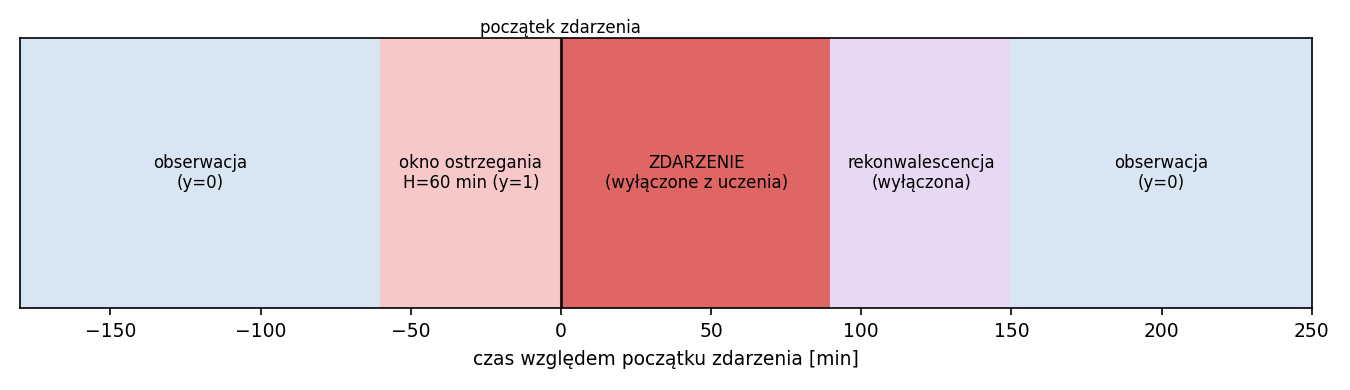
\includegraphics[width=\textwidth]{fig/schemat_etykiet.png}
      {\scriptsize Etykieta: $y(t)=1$, gdy silny epizod zacznie się w~ciągu \sig{60~min}.}
    \end{column}
  \end{columns}
\end{frame}

% =====================================================================
\section{Rozwiązanie}

\begin{frame}{Inżynieria cech --- fizyka zaszyta w~liczbach}
  \begin{columns}[T]
    \begin{column}{0.5\textwidth}
      \textbf{39 cech, wyłącznie z~przeszłości} (brak wycieku przyszłości)
      \begin{itemize}\footnotesize
        \item poziomy, zmiany (15/30/60 min), średnie kroczące,
        \item wszystkie młyny sklejone w~jeden zbiór (cechy niezależne od numeru młyna).
      \end{itemize}
    \end{column}
    \begin{column}{0.5\textwidth}
      \textbf{Cechy fizyczne (sedno)}
      \begin{itemize}\footnotesize
        \item \sig{deficyt} $=\frac{\text{zadana}-\text{pomiar}}{\text{zadana}}$ wentylacji,
        \item \sig{drożność} $=\frac{\text{przepływ}}{\text{wyjście regulatora}}$ (proxy oporu),
        \item \sig{moc\_na\_węgiel} $=\frac{\text{moc młyna}}{\text{prędkość podajnika}}$,
        \item minuty wysycenia regulatora, niestabilność mocy (std 30 min).
      \end{itemize}
    \end{column}
  \end{columns}
  \vspace{0.5em}
  \begin{block}{Bilans zbioru}
    \footnotesize $\sim$131\,700 minut, \sig{300 minut pozytywnych (0,23\%)}, 5 silnych epizodów --- klasa skrajnie rzadka.
  \end{block}
\end{frame}

\begin{frame}{Model i~walidacja}
  \begin{columns}[T]
    \begin{column}{0.5\textwidth}
      \textbf{Wybór: \sig{LightGBM} + reguła fizyczna}
      \begin{itemize}\footnotesize
        \item gradient boosting na cechach fizycznych: interpretowalny, trenuje się w~sekundy na CPU,
        \item reguła fizyczna jako \sig{niezależny watchdog} (poziom odniesienia).
      \end{itemize}
      \vspace{0.4em}
      \textbf{Dlaczego nie sieć głęboka?}
      \begin{itemize}\footnotesize
        \item \sig{5 zdarzeń / 1 miesiąc} --- o 1--2 rzędy za mało na deep learning,
        \item GPU zbędne (dane miesiąca $\sim$40 MB).
      \end{itemize}
    \end{column}
    \begin{column}{0.5\textwidth}
      \textbf{Uczciwa walidacja}
      \begin{itemize}\footnotesize
        \item \sig{leave-one-day-out} (27 foldów, grupowanie po dniach) $\Rightarrow$ brak wycieku czasowego,
        \item cechy liczone tylko z~przeszłości,
        \item wykluczone: postoje, 60 min po rozruchu, epizod + rekonwalescencja.
      \end{itemize}
      \vspace{0.4em}
      \textbf{Tłumienie fałszywych alarmów}
      \begin{itemize}\footnotesize
        \item alarm dopiero po \sig{3 kolejnych minutach} score $\ge$ próg.
      \end{itemize}
    \end{column}
  \end{columns}
\end{frame}

\begin{frame}{Identyfikacja obiektu --- zapchanie = spadek wzmocnienia}
  \begin{columns}[T]
    \begin{column}{0.6\textwidth}
      \centering
      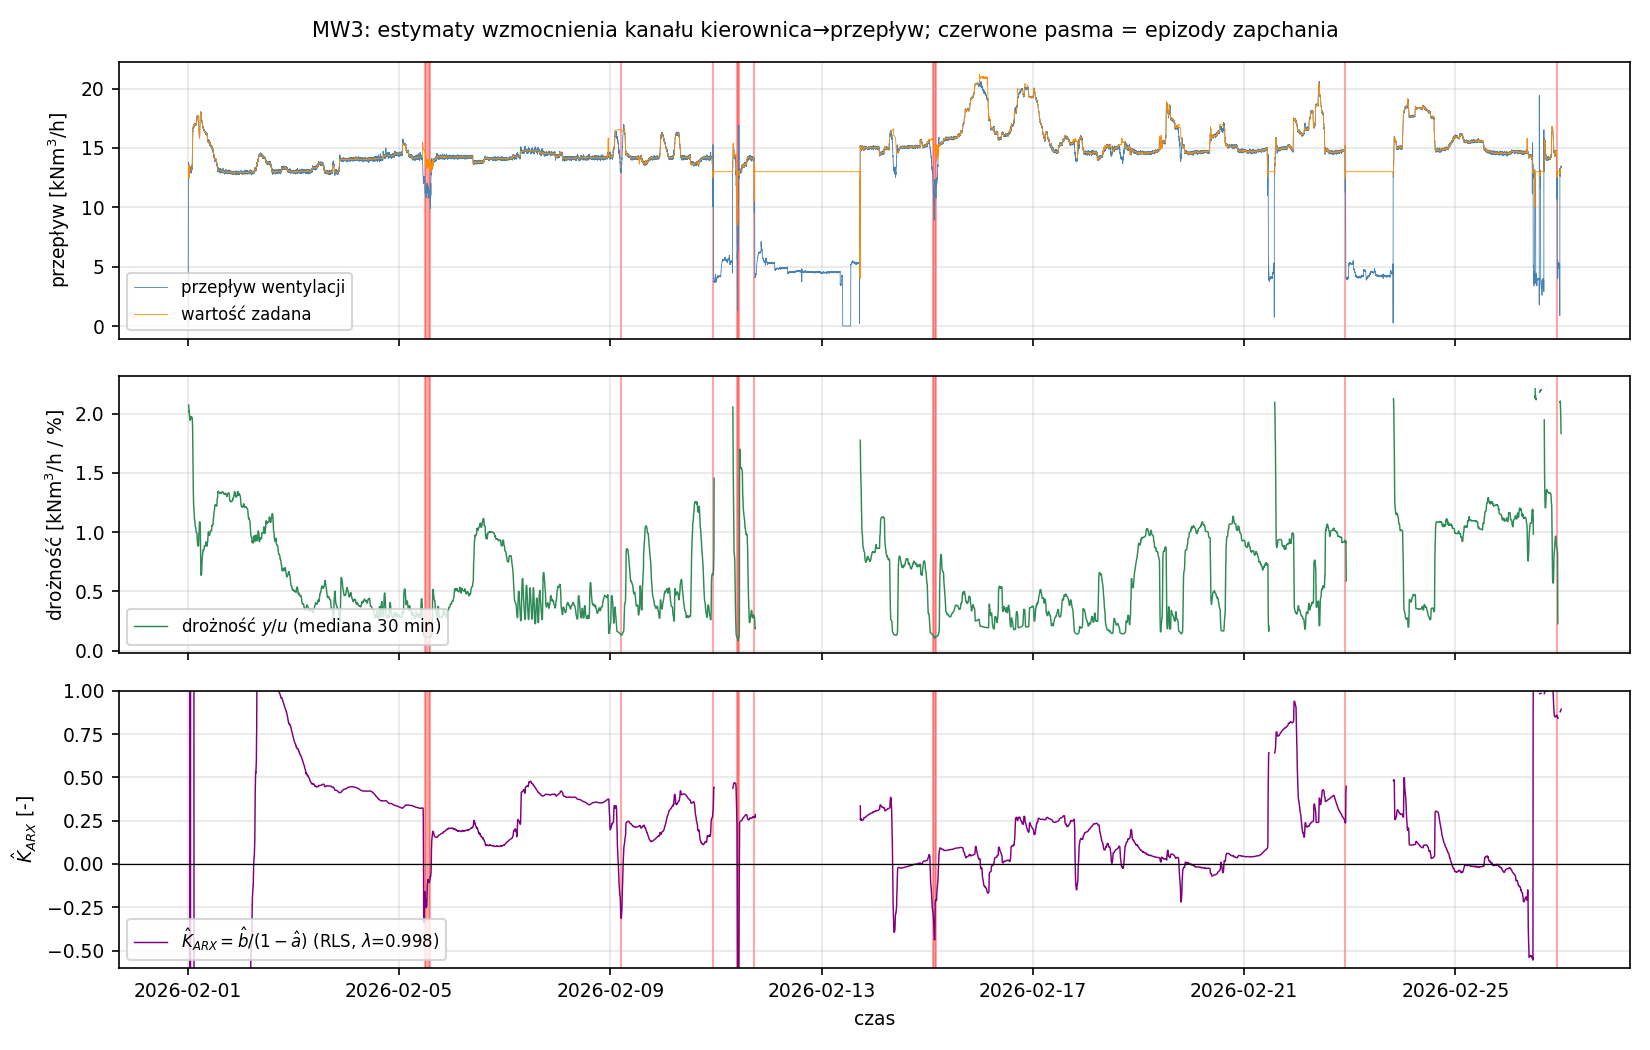
\includegraphics[width=\textwidth]{fig/identyfikacja_dryf_K_MW3.png}
    \end{column}
    \begin{column}{0.4\textwidth}
      \footnotesize
      Kanał \sig{kierownica $\to$ przepływ} traci wzmocnienie statyczne (drożność $y/u$) tuż przed epizodem:
      \vspace{0.3em}
      \begin{center}\scriptsize
      \begin{tabular}{lcc}
        \toprule
        młyn & zdrowy & przed \\
        \midrule
        MW3 & 0,506 & 0,277 \ (-45\%) \\
        MW4 & 0,917 & 0,152 \ (-83\%) \\
        \bottomrule
      \end{tabular}
      \end{center}
      \vspace{0.3em}
      Tor temperatury (FOPDT, pętla zamknięta): MW3 $K\!\approx\!1$, $T\!\approx\!23$~min.
      To \emph{ten sam} sygnał, który widzi model.
    \end{column}
  \end{columns}
\end{frame}

% =====================================================================
\section{Wyniki}

\begin{frame}{Wyniki --- porównanie modeli}
  \centering
  \renewcommand{\arraystretch}{1.25}
  \resizebox{\textwidth}{!}{%
  \footnotesize
  \begin{tabular}{lccccc}
    \toprule
    Model & PR-AUC & ROC-AUC & Epizody & Śr. wyprz. [min] & Fałsz./dobę/młyn \\
    \midrule
    reguła fizyczna            & ---   & ---   & \textbf{5/5} & \textbf{48,8} & 0,074 \\
    LightGBM (cechy, 5-fold)   & 0,286 & 0,931 & 4/5          & 33,0          & \textbf{0,046} \\
    \rowcolor{akcent!15}
    LightGBM, LODO (27 foldów) & 0,359 & 0,953 & \textbf{5/5} & 30,0          & 0,056 \\
    hybryda (LightGBM $\lor$ reguła), LODO & --- & --- & \textbf{5/5} & \textbf{51,0} & 0,093 \\
    \bottomrule
  \end{tabular}}
  \vspace{0.8em}
  \begin{itemize}\footnotesize
    \item Model finalny (LODO, próg 0,5, alarm po 3 min): \sig{5/5 epizodów, śr. 30 min wyprzedzenia, 0,056 fałszywej serii/dobę/młyn}.
    \item Hybryda z~regułą wydłuża wyprzedzenie do \sig{$\sim$51 min} kosztem nieco większej liczby fałszywych alarmów.
    \item Surowy klasyfikator minutowy jest słaby (PR-AUC $\sim$0,36 przy 0,23\% klasy) --- siła leży w~\emph{post-processingu} (próg + seria 3 min).
  \end{itemize}
\end{frame}

\begin{frame}{Jak to wygląda w~działaniu (walidacja LODO)}
  \centering
  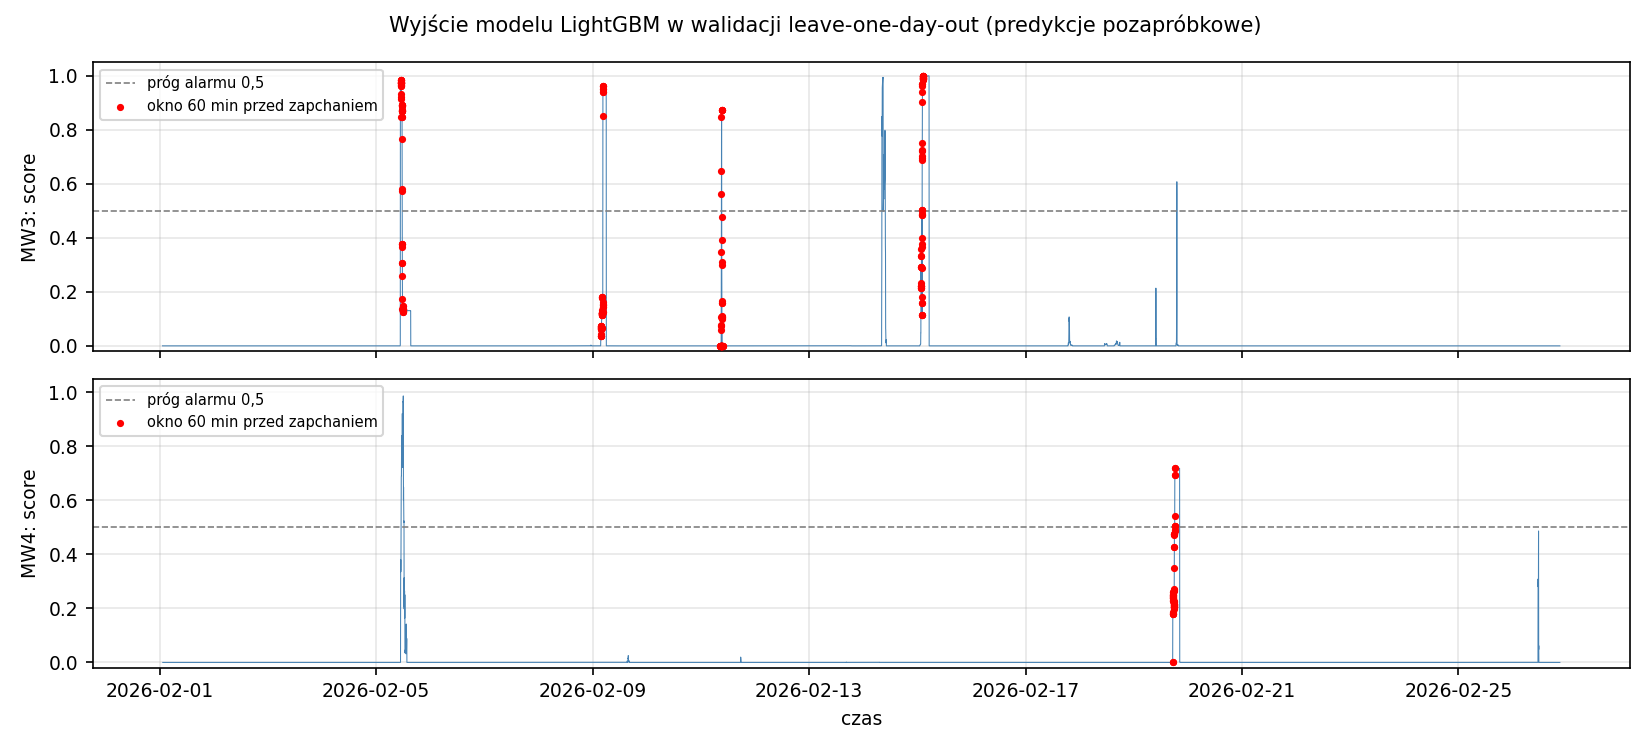
\includegraphics[width=0.96\textwidth]{fig/score_oof.png}
  {\scriptsize Wyjście modelu LightGBM (out-of-fold) dla MW3 i~MW4: szpilki score wyprzedzają pionowe znaczniki epizodów.}
\end{frame}

\begin{frame}{Co model faktycznie "widzi"}
  \begin{columns}[T]
    \begin{column}{0.58\textwidth}
      \centering
      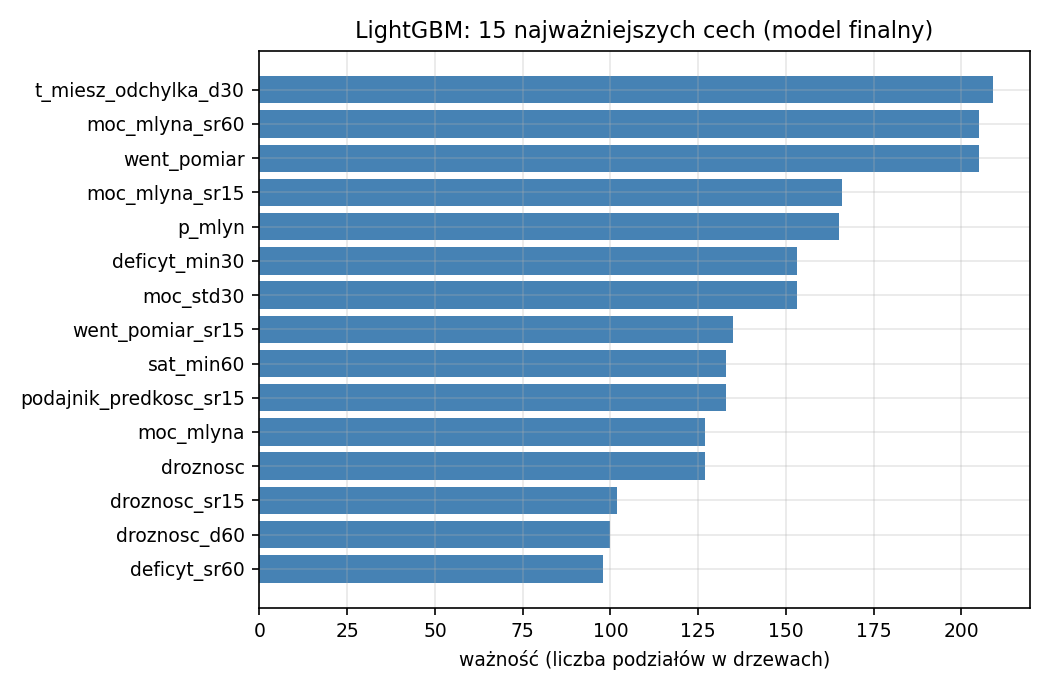
\includegraphics[width=\textwidth]{fig/waznosci_cech.png}
    \end{column}
    \begin{column}{0.42\textwidth}
      \footnotesize
      Najważniejsze cechy:
      \begin{itemize}\footnotesize
        \item pomiar przepływu wentylacji (poziom i~średnia 15 min),
        \item średnia moc młyna (60 min),
        \item zmiana odchyłki temperatury mieszanki (30 min),
        \item minuty deficytu, niestabilność mocy, drożność.
      \end{itemize}
      \vspace{0.4em}
      Wszystkie czołowe cechy mają \sig{jasną interpretację fizyczną} --- model zgadza się z~analizą identyfikacyjną.
    \end{column}
  \end{columns}
\end{frame}

\begin{frame}{Sieci neuronowe --- świadomy kontrprzykład}
  \begin{columns}[T]
    \begin{column}{0.62\textwidth}
      \centering
      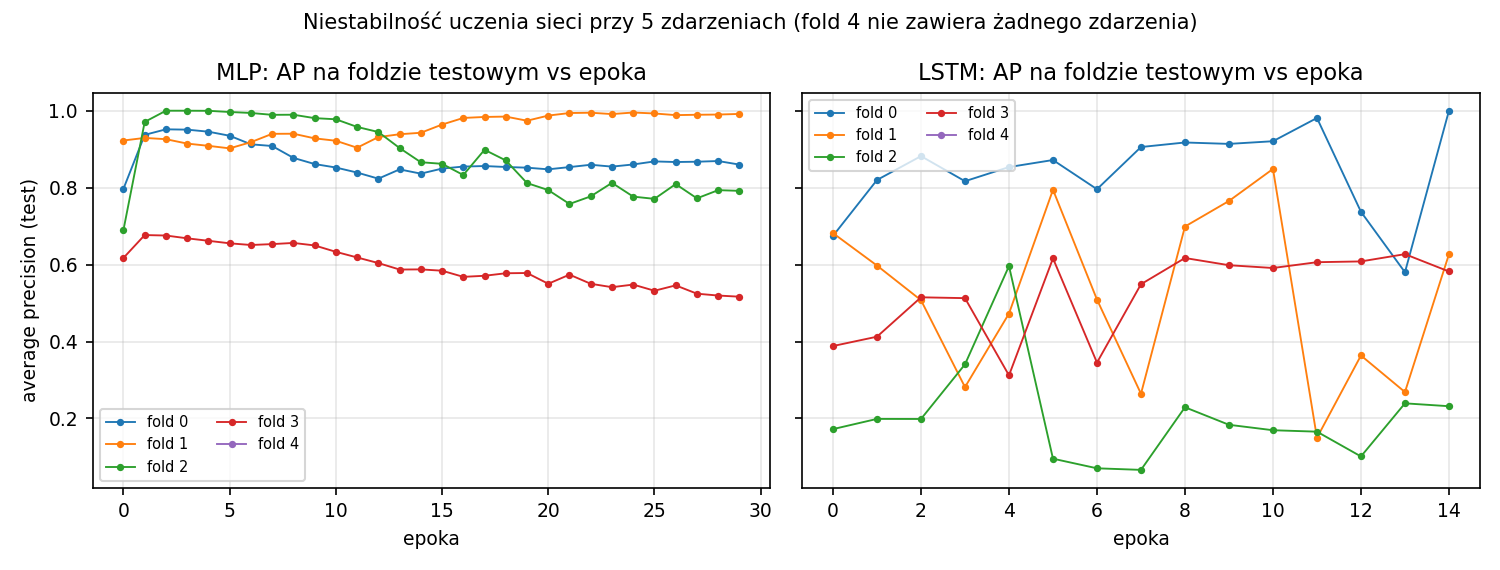
\includegraphics[width=\textwidth]{fig/krzywe_uczenia_nn.png}
    \end{column}
    \begin{column}{0.38\textwidth}
      \footnotesize
      MLP i~LSTM przy identycznej walidacji:
      \begin{itemize}\footnotesize
        \item \sig{brak spójnej przewagi} nad LightGBM,
        \item uczenie \sig{niestabilne} (krzywe skaczą --- za mało zdarzeń),
        \item zdarzeniowo podobna wykrywalność, ale więcej fałszywych alarmów.
      \end{itemize}
      \vspace{0.3em}
      Wniosek: przy 5 zdarzeniach \emph{prostszy, fizyczny} model wygrywa.
    \end{column}
  \end{columns}
\end{frame}

% =====================================================================
\section{Podsumowanie}

\begin{frame}{Ograniczenia i~co dalej}
  \begin{columns}[T]
    \begin{column}{0.5\textwidth}
      \textbf{Ograniczenia (uczciwie)}
      \begin{itemize}\footnotesize
        \item etykiety \sig{heurystyczne} --- wymagają potwierdzenia przez obsługę bloku,
        \item \sig{5 zdarzeń / 1 miesiąc / 2 młyny} --- na granicy istotności statystycznej,
        \item to \emph{studium wykonalności}, nie model produkcyjny.
      \end{itemize}
    \end{column}
    \begin{column}{0.5\textwidth}
      \textbf{Co dalej}
      \begin{itemize}\footnotesize
        \item 6--12 miesięcy danych (sezonowość, wilgotność węgla),
        \item dołączyć dane ogólnokotłowe i~KPI (obciążenie bloku),
        \item wdrożenie online: cechy w~oknie kroczącym + reguła jako watchdog,
        \item przy $>$50 zdarzeniach --- testy modeli sekwencyjnych (TCN/LSTM).
      \end{itemize}
    \end{column}
  \end{columns}
\end{frame}

\begin{frame}{Wnioski}
  \begin{block}{Najważniejsze}
    \begin{itemize}\footnotesize
      \item Zapchanie ma \sig{powtarzalny, fizyczny przebieg} i~mierzalne prekursory 60--120 min wcześniej.
      \item Identyfikacyjnie: epizod = \sig{spadek wzmocnienia} kanału kierownica$\to$przepływ (MW3 $-45\%$, MW4 $-83\%$).
      \item Finalny model (LightGBM, 39 cech fizycznych, LODO): \sig{5/5 epizodów, śr. 30 min wyprzedzenia, 0,06 fałszywej serii/dobę/młyn}; hybryda z~regułą --- do $\sim$51 min.
      \item Sieci neuronowe nie dają przewagi przy tej liczbie zdarzeń.
    \end{itemize}
  \end{block}
  \vspace{0.5em}
  \centering \large \textcolor{akcent}{Dziękujemy --- pytania?}
\end{frame}

\end{document}
